\chapter{ITk}
\label{chap::QT}
\chapterquote{Bigger...}%
{Everyone when I ask them about the FCC}
As of the writing of this thesis The LHC, and the ATLAS detector, is currently in its Run-3 data taking stage which will provide more data for our measurements and analyse and providing more statistics for combination measurements across the data taking stages. The delivered luminosity and mean crossings per bunch are higher than Run-2, these numbers are dwarfed when compared to the Run-4, where the LHC will enter its High-Luminosity era (HL-LHC) where it will be delivering an integrated luminosity of 3000 fb$^{-1}$ over ten years of operation (2029-2039). With the increased luminosity, there will also be increased pile-up, comprising the readout rates and increased radiation. This all means that we will be operating in a nosier environment, major reforms to the detector need to take place in order to benefit fully from the HL-LHC era. The main upgrade for this time will be a new inner detector system, which will be replaced by an all silicon inner tracker (ITk). 
\section{The ITk}
The ITk is designed to replace the current ID for the HL-LHC era in Run-4. It will be an all silicon solution, that comprises a pixel \refs and a strip subsystem \refs. The pixel subsystem covers a pseudorapidity range of $|\eta|<4.0$ and consists of five flat barrel layers and five layers of inclined or vertical rings for forward region coverage. The strip subsystem spans $|\eta|<2.7$ and includes four strip layers in the barrel region and six disks in the endcaps, all using double-sided modules. The layout of these subsystems can be shown in figure \ref{fig:itk-layout-p-s}. The resulting upgrade is expected to increase the trigger rate from 100 kHz to 1 MHz \refs. Improved radiation hardness of the subsystems will allow for the ITk to preform better in the high radiation environment of the HL-LHC. The higher granularity of the subsystems will improve the spatial resolution over the current ID and improve the vertex reconstruction, enhancing the b-tagging and pile- up rejection. 
\begin{figure}
    \centering
    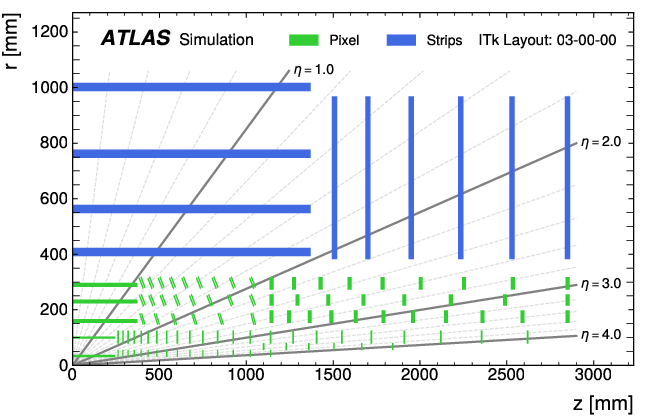
\includegraphics[width=1\linewidth]{Section_QT/itk-layout-p-s.png}
    \caption{}
    \label{fig:itk-layout-p-s}
\end{figure}
\subsection{Pixels}
The ITk pixel subsystem upgrade will consist of around 9400 modules and with 5 billion pixels covering an area of around 13 m$^2$. The Pixel subsystem layout is shown in figure \ref{fig:pixel-det-itk} and will be separated into three main zones the Inner System, Outer Rings and Outer Barrel. The Inner System consists of the Barrel with flat staves and Ring layers. The Pixel subsystem will use two main sensor technologies: Planar and 3D.
\\
\\
Planar technology is currently used in the pixel subsystem of the ID. For the ITk they have been redesigned in order to make them thinner and use n-in-p doping. There are many advantages for making the planar sensors thinner: we improve the radiation hardness, reduce the leakage current which helps with noise suppression, Improved response time, better track resolution and lower power consumption\refs. Planar sensors will be used in the outer rings and outer barrel regions.   
\\
\\
3D sensors are a type of silicon detector where electrodes (columns) are Etched into the silicon vertically, instead of being placed only on the surface like in planar sensors. This design allows for charge collection to happen in three dimensions, hence the name. As a result of the design, the 3D sensors have some unique benefits: The spacing of the electrodes are quite small resulting in shorter drift distances which reduces charge trapping. The charge collection time is also very short, improving time resolution and helping with pile up rejection\refs. The 3D sensors have improved radiation hardness compared to planar sensors making them ideal candidates for the inner-most part of the ITk, the Inner System.
\begin{figure}
    \centering
    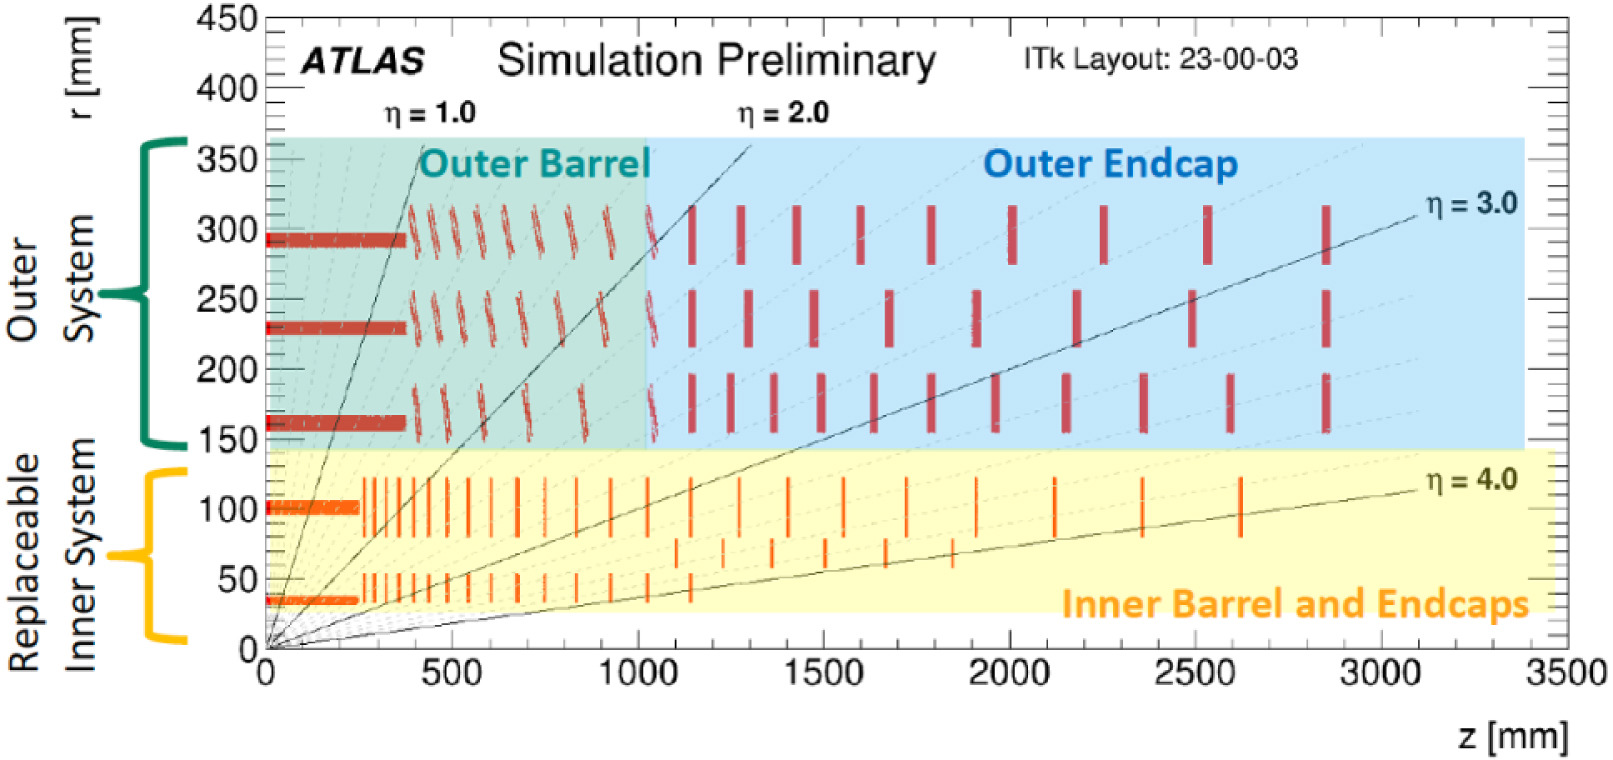
\includegraphics[width=0.75\linewidth]{Section_QT/pixel-det-itk.jpg}
    \caption{Enter Caption}
    \label{fig:pixel-det-itk}
\end{figure}
\subsection{Strips}
Surrounding the Pixel subsystem is the Strips subsystem, it is split into barrel and endcap regions. The barrel is made from four concentric layers, where the two layers closest to the collision point are made form short strip segments while the outer two layers are made from long strip sensors. 


\section{how we are building it and whos building it}
\subsection{problems with the global production line and why we need production tracking tools}
\section{ITk web app}
For my Qualification Task (QT) I was tasked with creating a tool in order to track the production rates of various components for the ITk upgrade, the components will undergo various testing before they are seen fit to be assembled into larger modules to then make it into the ITk. The official description of my task is as follows:

\begin{quote}
    The task will perform a regular query of the ATLAS ITk Production Database to understand the parts (e.g., modules) in different sites and compare to the production model. This information will then be used to guide the activity coordinators and the production managers in the decisions around part flow. For example, we will be able to see the number of modules in the different production sites and the need for modules at the different loading sites and compare to plan and act upon variance. A proposed weekly (frequency to be defined) job will perform the query, tabulate the data, and generate standard plots for the users. Access will be via a Web App. The tabulated data will be stored so that a history file will be created to allow time dependent analysis to be performed to understand groups production rates as well as part count on a given week. The tool and its use will be presented at the DB meeting. This task is useful both for Pixel and Strip.
    
\end{quote}
This tool will proved global value across the ITk production group. For the remainder of this chapter I shall focus on the UK-CHINA cluster and strips production. However, the web app frame work can be used for global (several clusters), individual cluster and local institution monitoring for both strips and pixels. 
\subsection{data pipelines}
Information about the location of the components and at which stage of testing or assembly they are in is contained in the ITk Production Database (PD). The PD however dose not provide timestamping, this is a crucial piece of information in order to produce the production timelines. In order to combat this short fall we need to timestamp these components ourselves. Timestamping the individual components would result in a lot of data points to manage as there could be thousands of the same components at the same testing or assembly stage. To reduce the number of data point, we consider the population of the components per stage. This will allow us to visualise the time line of a batch of components going through the various stages of testing or assembly and if any components fail the assembly or testing stages and thus deduce the yield and rate of production. 
\\
\\
Influxdb \cite{influx} was used to create timestamps of component stage populations. Influxdb is a third party timestamping data base, as data is fed into the db, it is then timestamped at the time of entry. Once the data is time stamped it can be readout using the inbuilt API. From here we can transform the raw timestamped data into our desired format and then plot. For plotting, we used Altair\cite{altair} a python based graphing package that offered the interactive functionality we needed to make a user friendly experience.
\\
\\
For this stage of development various versions of the interactive plot objects were prototyped and refined with feedback from institutes in the UK-China cluster. This refinement allowed for key performance indicators to be visualised within the plots. The finalised plot objects were then embedded in a web app hosted at CERN, allowing for all the institutes in the UK-CHINA cluster to access no only their own production time lines but also each others, meaning that all the production timeline information for each type of strips related component at all stages in all institutes where concatenated in one place. Using RedHat, for hosting and resource management, which pulled a series of Docker configs for containerisation. The Docker configs were stored securely on CERNs gitlab. Once the container was spun up, the web app is able to be hosted and accessed by anyone on the web, provided they have a access to the PD as access is password protected. 
A flowchart depicting the data pipeline for the web app is show in Fig.\ref{fig:datapipline}.
\begin{figure}[h!]
    \centering
    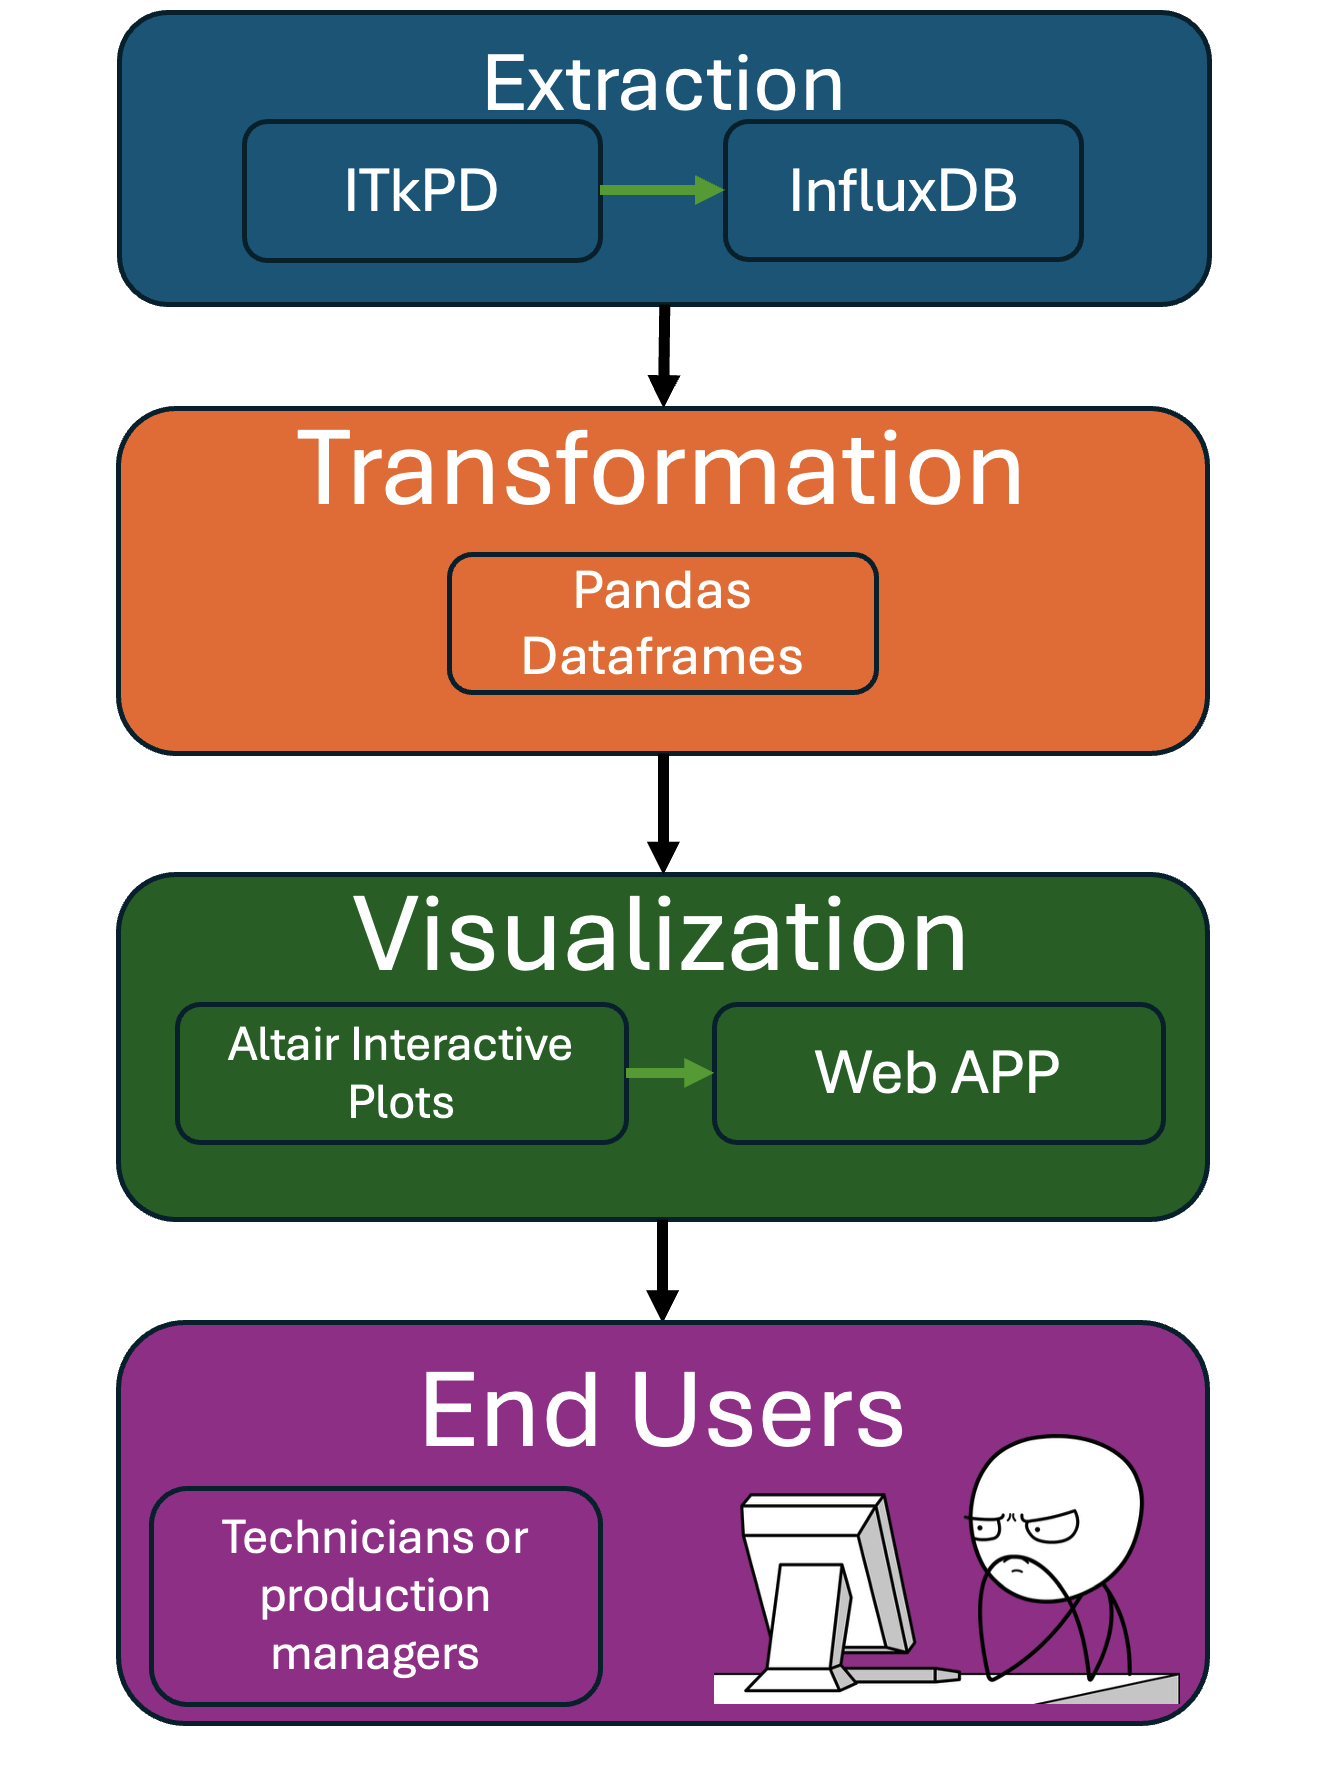
\includegraphics[width=0.5\linewidth]{Section_QT/data_pipline_qt.png}
    \caption{Enter Caption}
    \label{fig:datapipline}
\end{figure}
\\
\\
\subsection{Example interactive plots}
Below in Fig \ref{fig:web_app_plot_beta} is one of the early interactive plot prototypes. At the beginning of this project the ITk production was still in its relative infancy so only very technical institutes could contribute to the production and testing of components. One of these institutes was the Rutherford Appleton Laboratory (RAL). The large volume of components at RAL allowed for it to provide an ideal data set for the visualisation of components populations and the stage migration of these components. 
\begin{figure}[h!]
    \centering
    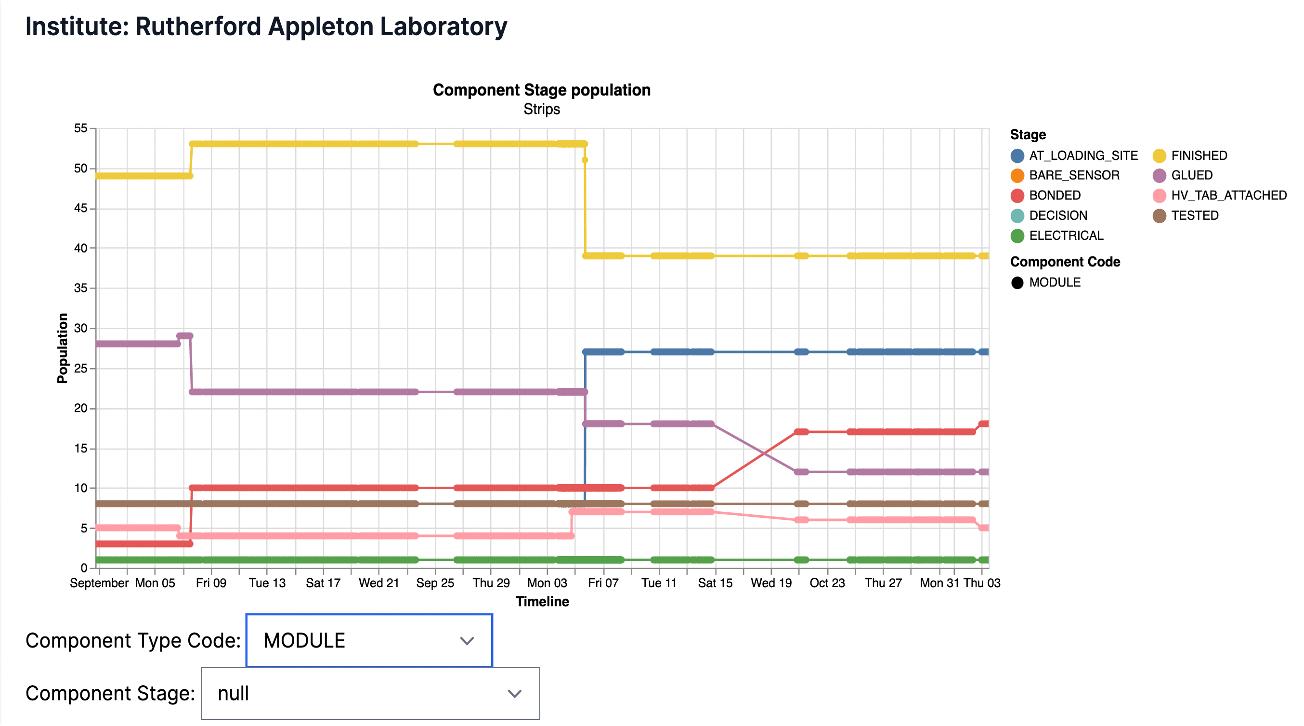
\includegraphics[width=1\linewidth]{Section_QT/web_app_plot_beta.png}
    \caption{Enter Caption}
    \label{fig:web_app_plot_beta}
\end{figure}
We see that in Fig. \ref{fig:web_app_plot_beta} we are only plotting modules and the components associated with them. This plot was made with an early build of the framework described in Fig.\ref{fig:datapipline}, even still we see that we managed to capture and visualise some batched of components transitioning through stages. For example we see various interplay between Glued (red) and Bonded (purple) as once the modules are glued to the stave the can be considered bonded.
\\
\\
This plot was then modified to include more component types, their stages and if the components had been trashed or not, as showed in Fig \ref{fig:ox_web_app}. 
\begin{figure}[h!]
    \centering
    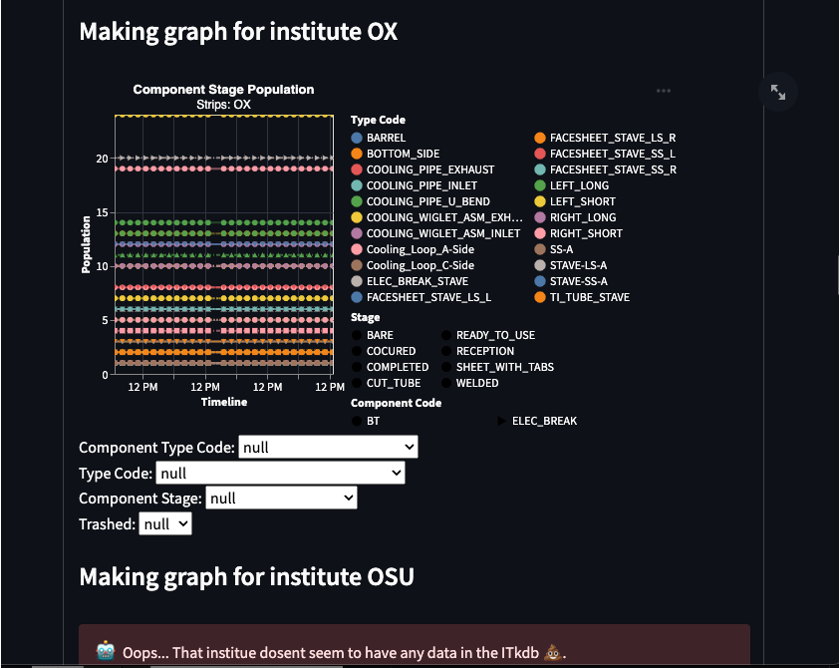
\includegraphics[width=0.8\linewidth]{Section_QT/ox_web_app.png}
    \caption{Enter Caption}
    \label{fig:ox_web_app}
\end{figure}
\subsection{rates}
\subsection{web app deployment and problems it solves}
